% ----------------------------------------------------------
\chapter{Metodologia para determinação dos esforços aerodinâmicos e matrizes \textbf{AIC}s}   %Apenas a primeira letra deve ser maiúscula
% ----------------------------------------------------------

As matrizes aerodinâmicas \gls{AICa} e \gls{AICc} foram determinadas utilizando-se da metodologia apresentada por \textcite{book:Bisplinghoff} utilizando as funções de \textit{Theodorsen} para uma seção típica bidimensional. A função de Theodorsen $C(k)$ adiciona os efeitos não-estacionários aos esforços aerodinâmicos atuando sobre a seção típica devido à dependência da frequência reduzida. O comportamento da função $C(k)$ é dado conforme mostrado na Figura \ref{fig:Theodorsen}.

\begin{figure}[ht!]
    \centering
    \caption{Função de Theodorsen $C(k)$ dependente da frequência reduzida}
    \noindent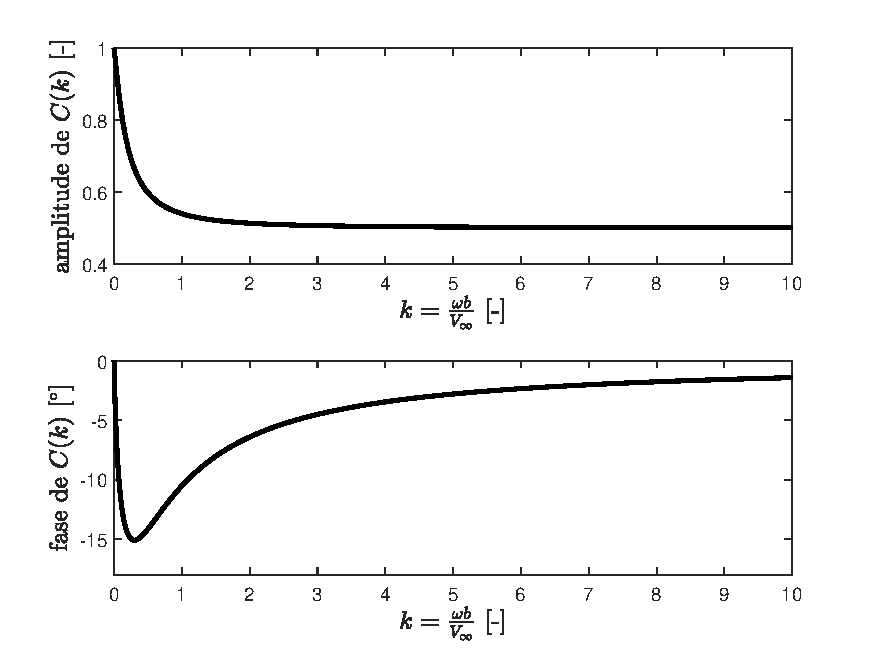
\includegraphics[width=\textwidth]{trabalho-graduacao/capitulos/figures/apendice/theodorsen.pdf}
    \label{fig:Theodorsen}
\end{figure}

Os esforços atuantes no sistema descrito na seção \ref{sec:descricao-sistema} são a sustentação $l$ e momento em torno do eixo elástico $m_{ea}$. Ambos esforços são dependentes dos parâmetros geométricos do sistema, das condições de voo para a qual são calculadas e da função de \textit{Theodorsen}. Matematicamente, são representados como

\begin{equation}\label{eq:sustentacao}
    l = 2\pi\gls{rho}\gls{Voo}\gls{b}QC(k) + \pi\gls{rho}\gls{b}^{2}\left[ \ddot{\gls{h}} + \gls{Voo}\dot{\gls{theta}} - \gls{b}\gls{a}\ddot{\gls{theta}} \right] + l_{\delta}
\end{equation}

\begin{multline}\label{eq:momento-ea}
    m_{ea} = -2\pi\gls{rho}\gls{Voo}\gls{b}^{2}Q\left\{ \frac{1}{2} - \left( a + \frac{1}{2} \right)C(k) \right\} \\ + \pi\gls{rho}\gls{b}^{2}\left[ \gls{Voo}\dot{\gls{h}} + \gls{b}\gls{a}\ddot{\gls{h}} + \gls{Voo}^{2}\gls{theta} - \gls{b}^{2}\left( \frac{1}{8}+\gls{a}^{2} \right) \ddot{\gls{theta}} \right] + m_{\delta}^{ea}
\end{multline}

\noindent em que $Q$ é uma função dependente do movimento oscilatório dos \gls{GDL}s do sistema e é dada por

\begin{multline}\label{eq:funcaoQ}
    Q = \gls{Voo}\gls{theta} + \dot{\gls{h}} + \gls{b}\left( \frac{1}{2} - \gls{a} \right)\dot{\gls{theta}} + \gls{delta}\frac{\gls{Voo}}{\pi}\left[ \sqrt{1-\gls{e}^{2}} + \cos^{-1}{\gls{e}} \right] \\ + \dot{\gls{delta}}\frac{\gls{b}}{2\pi}\left[ \left( 1 - 2\gls{e} \right)\cos^{-1}{\gls{e}} + (2-\gls{e})\sqrt{1-\gls{e}^{2}}\right]  
\end{multline}

Nas definições dos esforços aerodinâmicos em \eqref{eq:sustentacao} e \eqref{eq:momento-ea}, nota-se os termos da sustentação e momento em torno do eixo elástico decorrente da deflexão da superfície de controle, respectivamente $l_{\delta}$ e $m_{\delta}^{ea}$. Essas parcelas são calculadas como


\begin{align}\label{eq:sustentacao-delta}
\begin{split}
    l_{\delta} = &-\gls{rho}\gls{b}^{2}\gls{Voo} \left[ \gls{e}\sqrt{1-\gls{e}^{2}}-\cos^{-1}{\gls{e}} - \cos^{-1}{\gls{e}} \right]\dot{\gls{delta}} \\ &- \gls{rho}\gls{b}^{3}\left[ \gls{e}\cos^{-1}{\gls{e}} - \frac{1}{3}\left(2 + \gls{e}^{2} \right)\sqrt{1-\gls{e}^{2}} \right]\ddot{\gls{delta}}
\end{split}
\end{align}

\begin{align}\label{eq:momento-delta}
\begin{split}
    m_{\delta}^{ea} = &-\gls{rho}\gls{b}^{2}\gls{Voo}^{2} \left[ \gls{e}\sqrt{1-\gls{e}^{2}}-\cos^{-1}{\gls{e}} \right]\gls{delta} \\
        &-\gls{rho}\gls{b}^{3}\gls{Voo} \left\{ \frac{1}{3}\sqrt{1-\gls{e}^{2}}\left(\gls{e}^{2}-1\right) - \left(\gls{e}-\gls{a}\right)\left[ \gls{e}\sqrt{1-\gls{e}^{2}}-\cos^{-1}{\gls{e}} \right] \right\}\dot{\gls{delta}} \\
        &-\gls{rho}\gls{b}^{4}\left\{ \left(\frac{1}{8}+\gls{e}^{2}\right)\cos^{-1}{\gls{e}} -  \frac{1}{8}\gls{e}\sqrt{1-\gls{e}^{2}}\left(7+2\gls{e}^{2}\right) \right. \\ &+  \left. \left(\gls{e}-\gls{a}\right)\left[\frac{1}{3}\sqrt{1-\gls{e}^{2}}\left(2+\gls{e}^{2}\right) - \gls{c}\cos^{-1}{\gls{e}} \right] \right\} \ddot{\gls{delta}}
\end{split}
\end{align}

Substituindo \eqref{eq:funcaoQ}, \eqref{eq:sustentacao-delta} e \eqref{eq:momento-delta} em \eqref{eq:sustentacao} e \eqref{eq:momento-ea} é possível reescrever as expressões que indicam os esforços aerodinâmicos atuantes no sistema de forma matricial, como

\begin{equation}\label{eq:esforcos-matricial}
    \begin{bmatrix}
        l \\ m_{ea}
    \end{bmatrix} = 
    \boldsymbol{X}_{GDL,2}
    \begin{bmatrix}
        \ddot{\gls{h}} \\ \ddot{\gls{theta}}
    \end{bmatrix} +
    \boldsymbol{X}_{GDL,1}
    \begin{bmatrix}
        \dot{\gls{h}} \\ \dot{\gls{theta}}
    \end{bmatrix} +
    \boldsymbol{X}_{GDL,0}
    \begin{bmatrix}
        \gls{h} \\ \gls{theta}
    \end{bmatrix} +
    \boldsymbol{X}_{\delta,2}\ddot{\gls{delta}} + \boldsymbol{X}_{\delta,1}\dot{\gls{delta}} + \boldsymbol{X}_{\delta,0}\gls{delta}
\end{equation}

\noindent em que, $\boldsymbol{X}_{GDL,i}$ e $\boldsymbol{X}_{\delta,i}, \ i = 0,\ 1,\ 2$, representam as matrizes cujos termos são as parcelas que multiplicam cada variável dos \gls{GDL}s ou da deflexão da superfície de controle em \eqref{eq:sustentacao}, \eqref{eq:momento-ea}, \eqref{eq:funcaoQ}, \eqref{eq:sustentacao-delta} e \eqref{eq:momento-delta}. Aplicando a transformada de Laplace, \eqref{eq:esforcos-matricial} pode ser escrita como

\begin{equation}\label{eq:esforcos-matricial2}
    \begin{bmatrix}
        l \\ m_{ea}
    \end{bmatrix} = \left(
    \boldsymbol{X}_{GDL,2}s^{2} + \boldsymbol{X}_{GDL,1}s + \boldsymbol{X}_{GDL,0} \right)
    \begin{bmatrix}
        \gls{h}(s) \\ \gls{theta}(s)
    \end{bmatrix} +
    \left( \boldsymbol{X}_{\delta,2}s^{2} + \boldsymbol{X}_{\delta,1}s + \boldsymbol{X}_{\delta,0} \right) \gls{delta}(s)
\end{equation}

Utilizando da definição da frequência reduzida em \eqref{eq:Frequencia-reduzida}, pode reescrever \eqref{eq:esforcos-matricial2} como

\begin{align}\label{eq:esforcos-matricial3}
\begin{split}
    \begin{bmatrix}
        l \\ m_{ea}
    \end{bmatrix} = &\left(
    \left(\frac{\gls{Voo}}{b}\right)^{2}\boldsymbol{X}_{GDL,2}(ik)^{2} + \frac{\gls{Voo}}{b}\boldsymbol{X}_{GDL,1}(ik) + \boldsymbol{X}_{GDL,0} \right)
    \begin{bmatrix}
        \gls{h}(s) \\ \gls{theta}(s)
    \end{bmatrix} \\ &+
    \left( \left(\frac{\gls{Voo}}{b}\right)^{2}\boldsymbol{X}_{\delta,2}(ik)^{2} + \frac{\gls{Voo}}{b}\boldsymbol{X}_{\delta,1}(ik) + \boldsymbol{X}_{\delta,0} \right) \gls{delta}(s)
\end{split}
\end{align}

Analisando \eqref{eq:esforcos-matricial3} em comparação com o lado direito de \eqref{eq:equacao-dinamica-final}, percebe-se que, organizando os termos e colocando a pressão dinâmica $\gls{qoo}$ em evidência em \eqref{eq:esforcos-matricial3}, encontramos as matrizes $\gls{AICa}$ e $\gls{AICc}$ como

\begin{equation}\label{eq:AICa-definica}
    \gls{AICa} = \frac{1}{\gls{qoo}}\left(
    \left(\frac{\gls{Voo}}{b}\right)^{2}\boldsymbol{X}_{GDL,2}(ik)^{2} + \frac{\gls{Voo}}{b}\boldsymbol{X}_{GDL,1}(ik) + \boldsymbol{X}_{GDL,0} \right)
\end{equation}

\begin{equation}\label{eq:AICc-definica}
    \gls{AICc} = \frac{1}{\gls{qoo}}\left( \left(\frac{\gls{Voo}}{b}\right)^{2}\boldsymbol{X}_{\delta,2}(ik)^{2} + \frac{\gls{Voo}}{b}\boldsymbol{X}_{\delta,1}(ik) + \boldsymbol{X}_{\delta,0} \right)
\end{equation}
